\section{Methodology}\label{sec:methodology}

\subsection{Dataset}

Our dataset is derived from the publically available Face Research Lab London (FRLL)~\cite{DeBruine2017} set, comprising 102 frontal ICAO-compliant facial images. Each image was encoded using four printer-proof steganographic methods, described ahead, each applied at nine different intensity levels, yielding a total of 3,672 distorted images.

The dataset was partitioned into four subsets, as follows:

\begin{itemize}
    \item Labeled Set (15 identities, 540 images): a core set of demographically diverse subjects, shown in Fig.~\ref{fig:subdataset}, annotated with MOS through human evaluation.
    \begin{itemize}
        \item Training Subset (12 identities, 432 images): used to train the full-reference fusion model, regressing FR-IQA metrics to human MOS.\@
        \item Disjoint Test Subset (3 identities, 108 images): held out from the framework and are used solely for final results comparisons, simulating out-of-distribution generalization.
    \end{itemize}
    \item Unlabeled Set (87 identities, 3,132 images): no subjective scores were collected for these images. Instead, pseudo-MOS labels were generated using the FR fusion model, enabling large-scale weak supervision.
    \item No-Reference (NR) Training Pool (99 identities, 3,564 images): Combines the 12 labeled identities and the 87 pseudo-labeled identities, and is used to train the NR regression model on deep features extracted from distorted images.
\end{itemize}

\begin{figure}
    \centering
    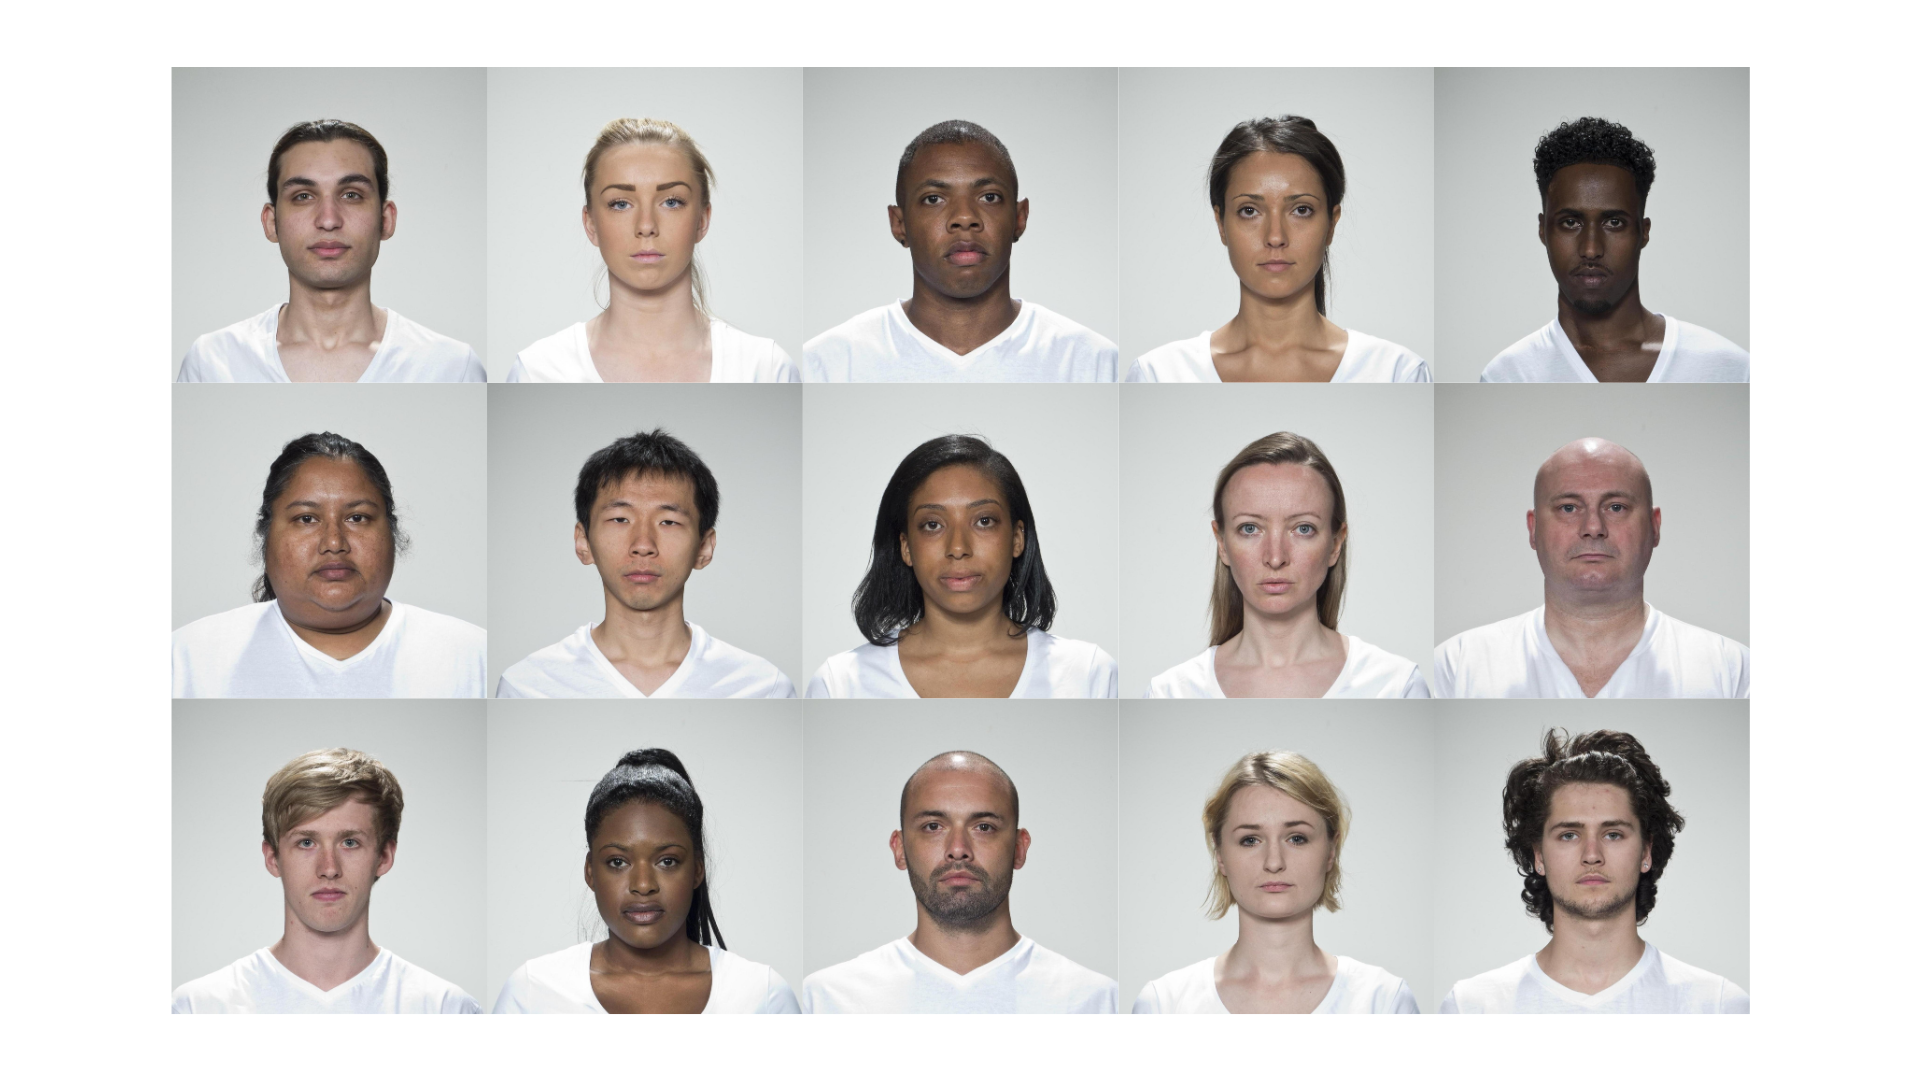
\includegraphics[width=1\linewidth]{images/subdataset.png}
    \caption{Labeled set selected from the FRLL dataset.}\label{fig:subdataset}
\end{figure}

The printer-proof steganography methods used were based on Generative Adversarial Networks (GANs)~\cite{gans2018} to encode and decode information, we can obtain various results depending on the method used:

\begin{itemize}
    \item StegaStamp~\cite{stegastamp2020}: claims to be the first steganography model capable of decoding data from printed images. The authors show robust results in decoding data under physical transmission by developing novel strategies to add noise in the training process, printer noise simulation, and distortion for the training dataset.
    \item CodeFace~\cite{codeface2021}: encoder and decoder networks are trained using end-to-end GANs. It introduces a new security system for encoding and decoding facial images that are printed in common IDs and MRTDs.
    \item RiemStega~\cite{cruz2025riemstega}: proposes a new loss function that extends the loss function based on the $L_2$ distance between images to the Riemannian manifold of symmetric and positive definite matrices.
    \item StampOne~\cite{stampone2023}: focuses on high-level robust steganography, such as~\cite{codeface2021, stegastamp2020}, striking a balance between high-quality encoded images and decoding accuracy. It mitigates distortion-related issues like JPEG compression, camera sensors and printer's Gaussian noise by incorporating gradient transform, wavelet transform, and Depthwise~\cite{tay2022efficient} to normalize and balance frequencies of the inputs. 
\end{itemize}

Each image in our dataset was evaluated approximately 30 times by human observers, providing a robust MOS dataset.

We followed ITU-R BT.500--15~\cite{ITU-R-BT500} recommendation, and adopted the Single Stimulus method. Around 200 different observers were carefully instructed on how to perform the test session, the average duration of the session was 22 minutes, and the rounded number of tests in each session was 70. Resulting in over 14,000 evaluations.

To conduct the sessions we created a webapp in Django, seen in Fig.~\ref{fig:platform}, where the observers were asked to evaluate each image on a scale from 1 to 100 using a slider bar, with no time limit. The rating scale was divided into five categorical levels: scores from 1 to 25 were classified as Bad, 26 to 50 as Poor, 51 to 75 as Fair, 76 to 99 as Good, and a score of 100 as Excellent.

\begin{figure}
    \centering
    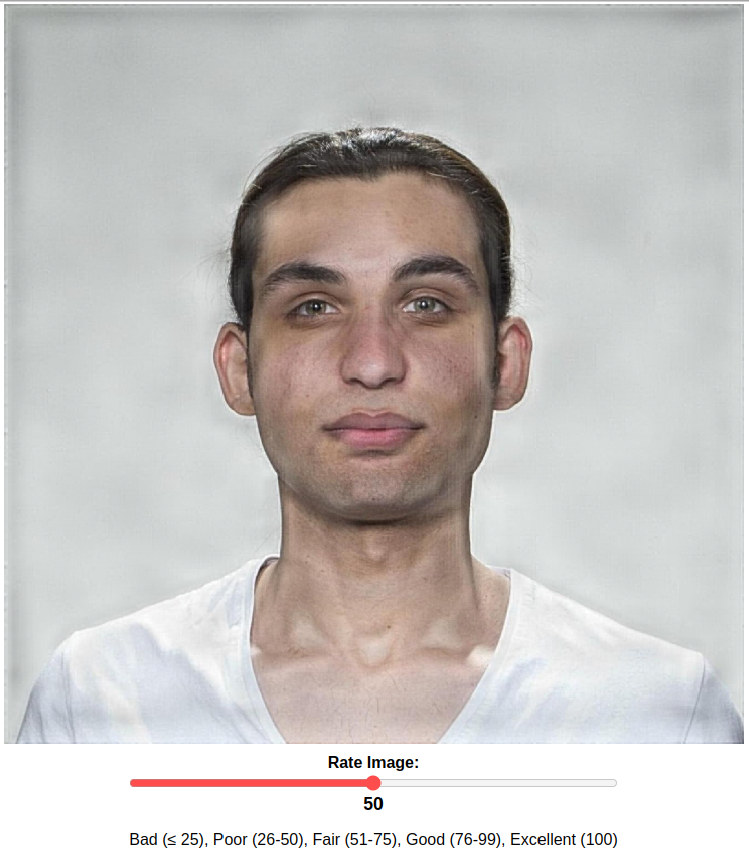
\includegraphics[width=0.4\linewidth]{images/webapp.png}
    \caption{Snippet of the custom webapp platform used to access overall image quality.}\label{fig:platform}
\end{figure}

%\subsection{Statistical Bias in Facial Quality Perception}

%Perceptual evaluation of facial image quality is inherently biased by observer characteristics. In facial imagery, these biases are amplified by the brain’s specialized processing of faces, where factors such as familiarity, symmetry, and subtle texture cues heavily influence perceived quality. Our earlier user studies revealed strong inter-observer variability when assessing steganographically distorted faces, highlighting that MOS are not purely determined by signal-level distortions but also by cognitive priors. This makes the design of facial-specific IQA systems particularly challenging.

To address this, we propose a two-stage hybrid pipeline that first builds a full-reference (FR) quality estimator supervised by MOS, and then extends this supervision to a no-reference (NR) model via pseudo-MOS learning.

\subsection{Full-Reference Analysis and Fusion}

We compute 41 FR-IQA scores for each distorted image in the MOS-labeled subset. To identify which metrics align best with human perception, we calculate both the Pearson Linear Correlation Coefficient (PLCC) and the Spearman Rank-Order Correlation Coefficient (SRCC)~\cite{plcc_srcc} between each metric and the human MOS.\@ This analysis serves to rank the metrics and select the top-$k$ most perceptually relevant.

\subsection{Pseudo-MOS Generation via FR-IQA Fusion}

The selected top-$k$ IQA metrics are standardized and used as input features for supervised regression models trained to approximate the human MOS.\@ We evaluate Support Vector Regression~\cite{svr}, Random Forest~\cite{randomforest}, XGBoost~\cite{xgboost}, and LightGBM~\cite{lightgbm} as candidate fusion models. Random Forest consistently achieved the highest PLCC and SRCC on the validation set for $k=5$, and was selected as the fusion model. This trained regressor is then applied to the unlabeled portion of the dataset (3,132 distorted images), generating pseudo-MOS scores that serve as proxy ground-truth labels.

\subsection{NR Regression Model}

To enable NR quality prediction, we extract deep features from each distorted image using a ResNet-18~\cite{resnet} model pretrained on ImageNet. These feature vectors are then used to train a regression model, again using Random Forest, tasked with predicting the pseudo-MOS labels obtained from the FR fusion step. The final model performs quality assessment using only the distorted input image, without requiring access to a reference image, thereby enabling NR-IQA in real-world scenarios.
